\documentclass[12pt]{article}
\usepackage[left=3cm, top=1cm, right=3cm, bottom=3cm]{geometry}
\usepackage[utf8]{inputenc}      % accents dans le source
\usepackage[T1]{fontenc}
\usepackage[french]{babel}
\usepackage{graphicx}
\usepackage{graphics}
\usepackage{amsmath}
\usepackage{tikz}
\usepackage{xcolor} 
\usepackage{mathtools}
\usepackage{parskip}
\usepackage{subcaption}
\usepackage[export]{adjustbox}
\usepackage{chemist}
\usepackage{rotating}
\usepackage{hyperref}
\hypersetup{colorlinks=true,linkcolor=blue}

\title{\textbf{TP1 Chimie Inorganique} \\ Complexes et couleur}
\author{MENARD Alexandre \\ VIEILLEDENT Florent}

\begin{document}
\maketitle

\section*{Introduction}

Dans ce travail pratique nous étudions la couleur de complexe de métaux de transitions.
Nous regardons l'influence de la géométrie et du ligand sur la couleur d'un complexe.
Nous réalisons le spectre d'absorbtion UV-visible pour déterminer la longueur d'onde absorbée par les complexes.

\section{Spectre UV-visible d'une solution de permanganate de potassium}

Dans cette expérience, nous réalions le spectre UV-visible d'un complexe de permanganate $[MnO_4]^-$ et nous déterminons la longeur d'onde $\lambda_{max}$ et le coefficient d'extionction molaire $\epsilon_{max}$.

\subsection{Protocole}

Une première solution de permanganate de concentration $c_0=4 \times 10^{-3} \ M $ est préparée en dissolvant $0.03 \ g$ de permanganate de potassium $KMnO_4$ dans de l'eau distillée dans une fiole jaugée de 50 mL.
La solution est ensuite diluée d'un facteur 10 en prélevant 10 mL qu'on introduit dans une fiole jaugée de 100 mL qu'on remplit ensuite avec de l'eau distillée.
La nouvelle concentration est $c=4 \times 10^{-4} \ M $.

\newpage
\subsection{Résultats}

On réalise le spectre UV-visible de notre solution de permanganate.
\begin{figure}[h!]
    \begin{center}
        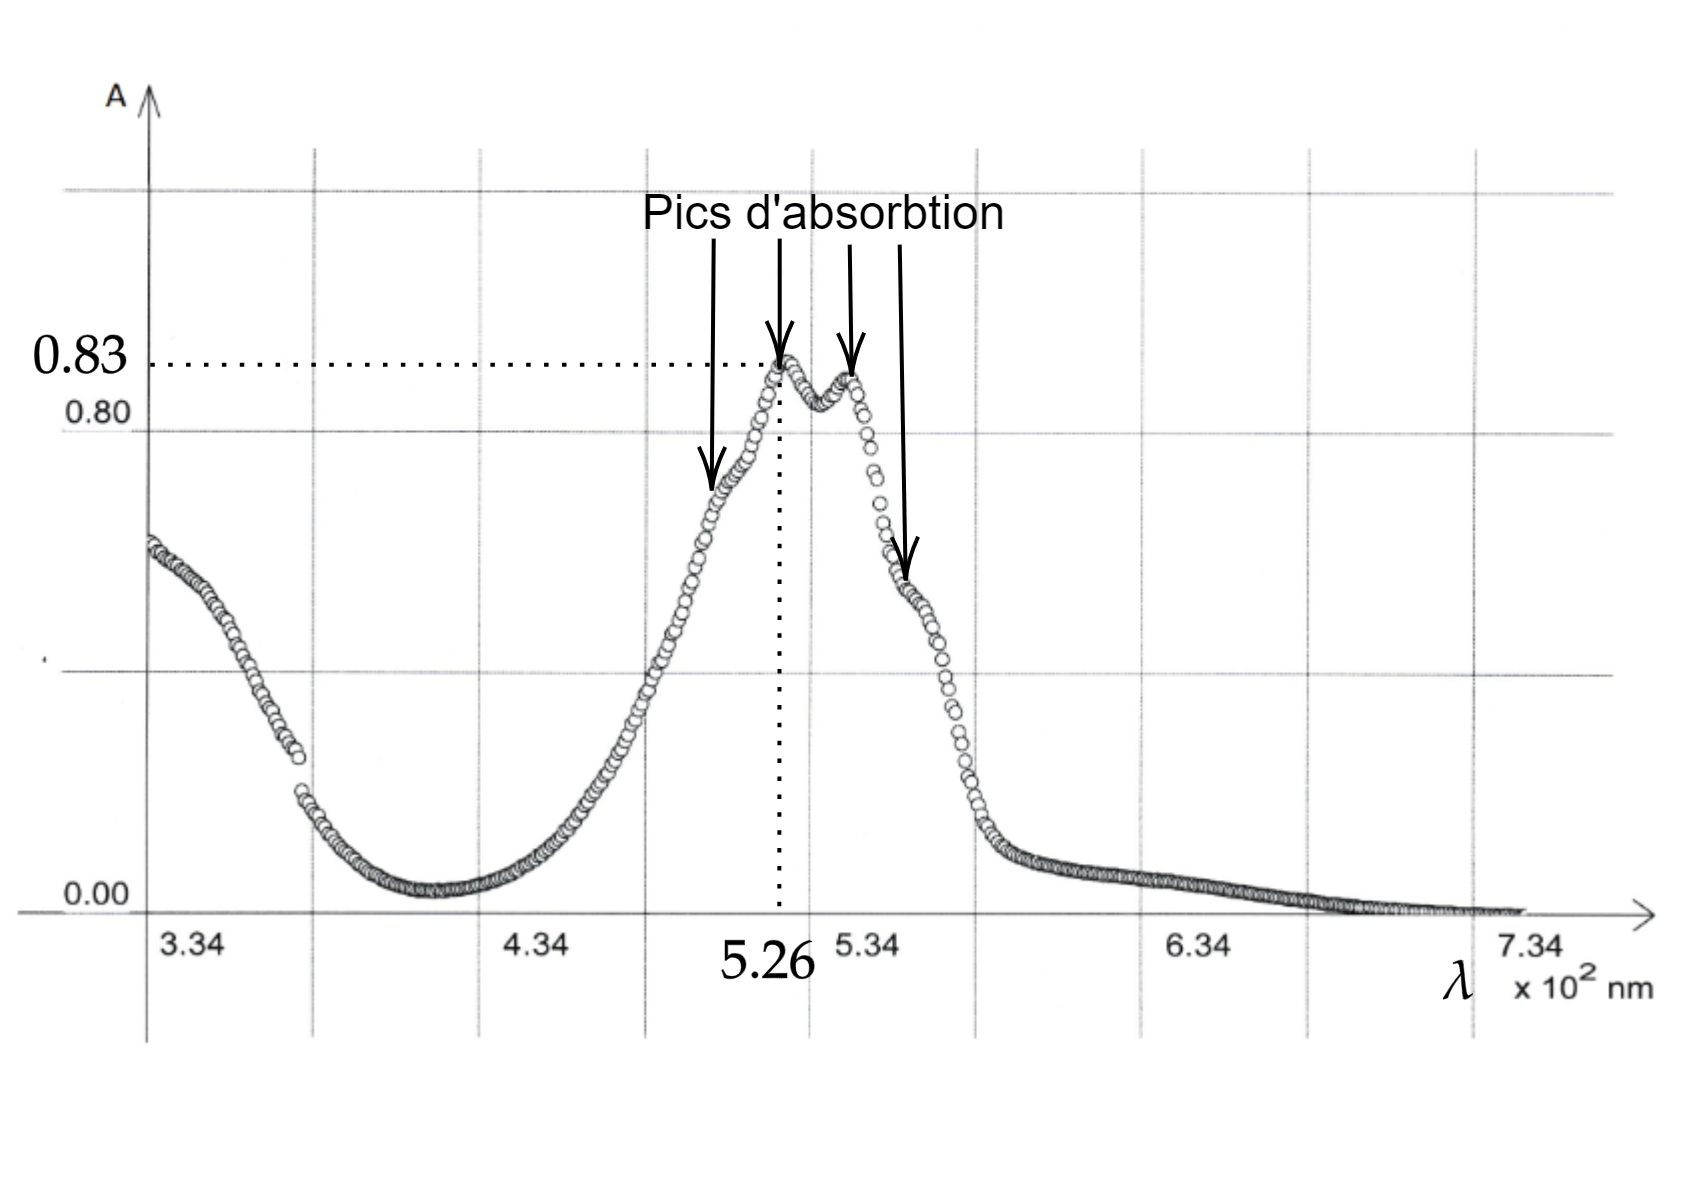
\includegraphics[scale=0.7]{Spectre1_Inorga_bis.jpeg}
        \caption{Graphique de l'aborbance de la solution de permanganate de concentration $10^{-4} \ M$ en fonction de la longueur d'onde}
        \label{img1:Spectre_permanganate}
    \end{center}
\end{figure}

On observe 4 pics d'absorbances. 

\subsection{Théorie et interprétations des résultats}

Dans le complexe permanganate, le manganèse $Mn$ est dans un état d'oxydation $+ VII$ et son $d^n=d^0$.
Comme il n'y a pas d'électrons dans les orbitales d du métal, aucune transition d-d n'est possible.
On peut toujours observer des transferts de charge du ligand au métal (LMCT). 

Comme il y a 4 atomes d'oxygène autour du métal, on peut s'attendre à 4 LMCT succéssifs, ce qui est en accord avec les 4 pics d'absorbances sur la figure (1).

On détermine la longueur d'onde absorbée $\lambda_{max}$ et le coefficient d'absorbtion molaire $\epsilon_{max}$ pour le plus grand pic d'absorbtion.
On obtient graphiquement $\lambda_{max}=526 \ nm$.
Pour déterminer $\epsilon_{max}$ on utilise la loi de Beer-Lambert:
\begin{align*}
    A=\epsilon_{max} \times c \times l &\Longrightarrow \epsilon_{max}=\frac{A}{c \times l} \\
      &\Longrightarrow \epsilon_{max}=\frac{0.93}{4 \times 10^{-4} \times 1} \\
      &\Longrightarrow \epsilon_{max}=2325 \ L.mol^{-1}.cm^{-1}
\end{align*}

On retrouve bien un $\epsilon > 1000 \ L.mol^{-1}.cm^{-1}$, ce qui est attendu pour un transfert de charge.

\section{Complexe de cobalt thermochrome : influence de la géométrie sur la couleur}

Dans cette expérience nous étudions l'effet de la température sur la couleur d'un complexe de cobalt. 

\subsection{Protocole expérimental}

0.6 g de chlorure de cobalt hexahydraté $COCl_2,6H_2O$ est dissout dans 5mL d'eau dans un bécher. 
20 mL d'acétone sont ajoutés à l'aide d'une éprouvette graduée.
La solution est refroidie dans un bain de glace, puis est chauffée dans un bain jusqu'à environ $50 ^\circ C$.

\subsection{Observations}

Avant l'ajout d'acétone on observe un rose/rouge intense. 
Apres l'ajout d'acétone et à basse température on observe quasiment la même couleur mais en moins intense.
À haute température on observe une couleur bleue foncée.

\subsection{Théorie et observation}

Le cobalt peut former deux complexes différents dans notre solution : un complexe octaédrique avec le ligand aqua $[Co(H_20)_6]^{2+}$ et un complexe tétraédrique avec le ligand chloro $[CoCl_4]^{2-}$.
Dans les deux complexes, l'atome de cobalt est dans un état d'oxydation $+II$ et a un $d^n=d^7$.
On peut calculer les énergies de stabilisation associées au 2 géométries : on obtient $ESCC(H20)=-\frac{4}{5} \Delta_O$ et $ESCC(CL)=-8/15 \Delta_O$.
Comme $ESCC(H_2O)<ESCC(Cl)$, le complexe avec le ligand aqua est plus stable, ce sera donc le complexe majoritaire à basse température.

On a la relation $\Delta_t=\frac{4}{9}\Delta_O$, on s'attend donc à ce que les longueurs d'ondes absorbées augmentent lorqu'on passe de la géométrie octaédrique à la géométrie tétraédrique. 

À basse température on observe une couleur rose/rouge, donc la couleur verte est absorbée ce qui corespond à une longeur d'onde absorbée $\lambda_1=530 nm$ et $\Delta=\frac{1}{530 \times 10^{-7}}=22200 \ cm^{-1}$.

À haute température on observe une couleur bleue, donc la couleur rouge est absorbée ce qui correspond à une longeur d'onde $\lambda_2=630 nm$ et $\Delta=15 900 \ cm^{-1}$.

On a bien $\lambda_1<\lambda_2$ comme ce qu'avait prédit la théorie.

\section{Série spectrochimique : influence du ligand sur la couleur}

Dans cette expérience on s'interesse à étudier l'influence du ligand sur la couleur d'un complexe de nickel.

\subsection{Protocol expérimental}

Une solution à 0.4 M de $Ni(NO_3)_2,6H_2O$ est préparée en dissolvant 5.79 g dans de l'eau distillée dans une fiole jaugée de 50 mL.
On remplit une première graduée avec cette solution et une autre burette avec une solution d'éthylène diamine (en) à 0.4 M.
On remplit 5 tubes à essais avec différentes proportions des 2 solutions.

\begin{table}[h!]
    \begin{center}
        \begin{tabular}{|c|c|c|}
            \hline
            Tube & Volume de $Ni(NO_3)_2,6H_2O$ (en ml) & Volume de en (en ml) \\
            \hline
            1 & 10 & 0 \\
            2 & 8 & 2 \\
            3 & 6.7 & 3.3 \\
            4 & 5 & 5 \\
            5 & 2 & 8 \\
            \hline
        \end{tabular}
        \caption{Table des volumes introduits dans les tubes à essais}
        \label{table1:volume}
    \end{center}
\end{table}

\newpage
\subsection{Observations}
On réalise les spectres d'absorbtion UV-visible des différentes solutions.

\begin{figure}[h!]
    \begin{center}
        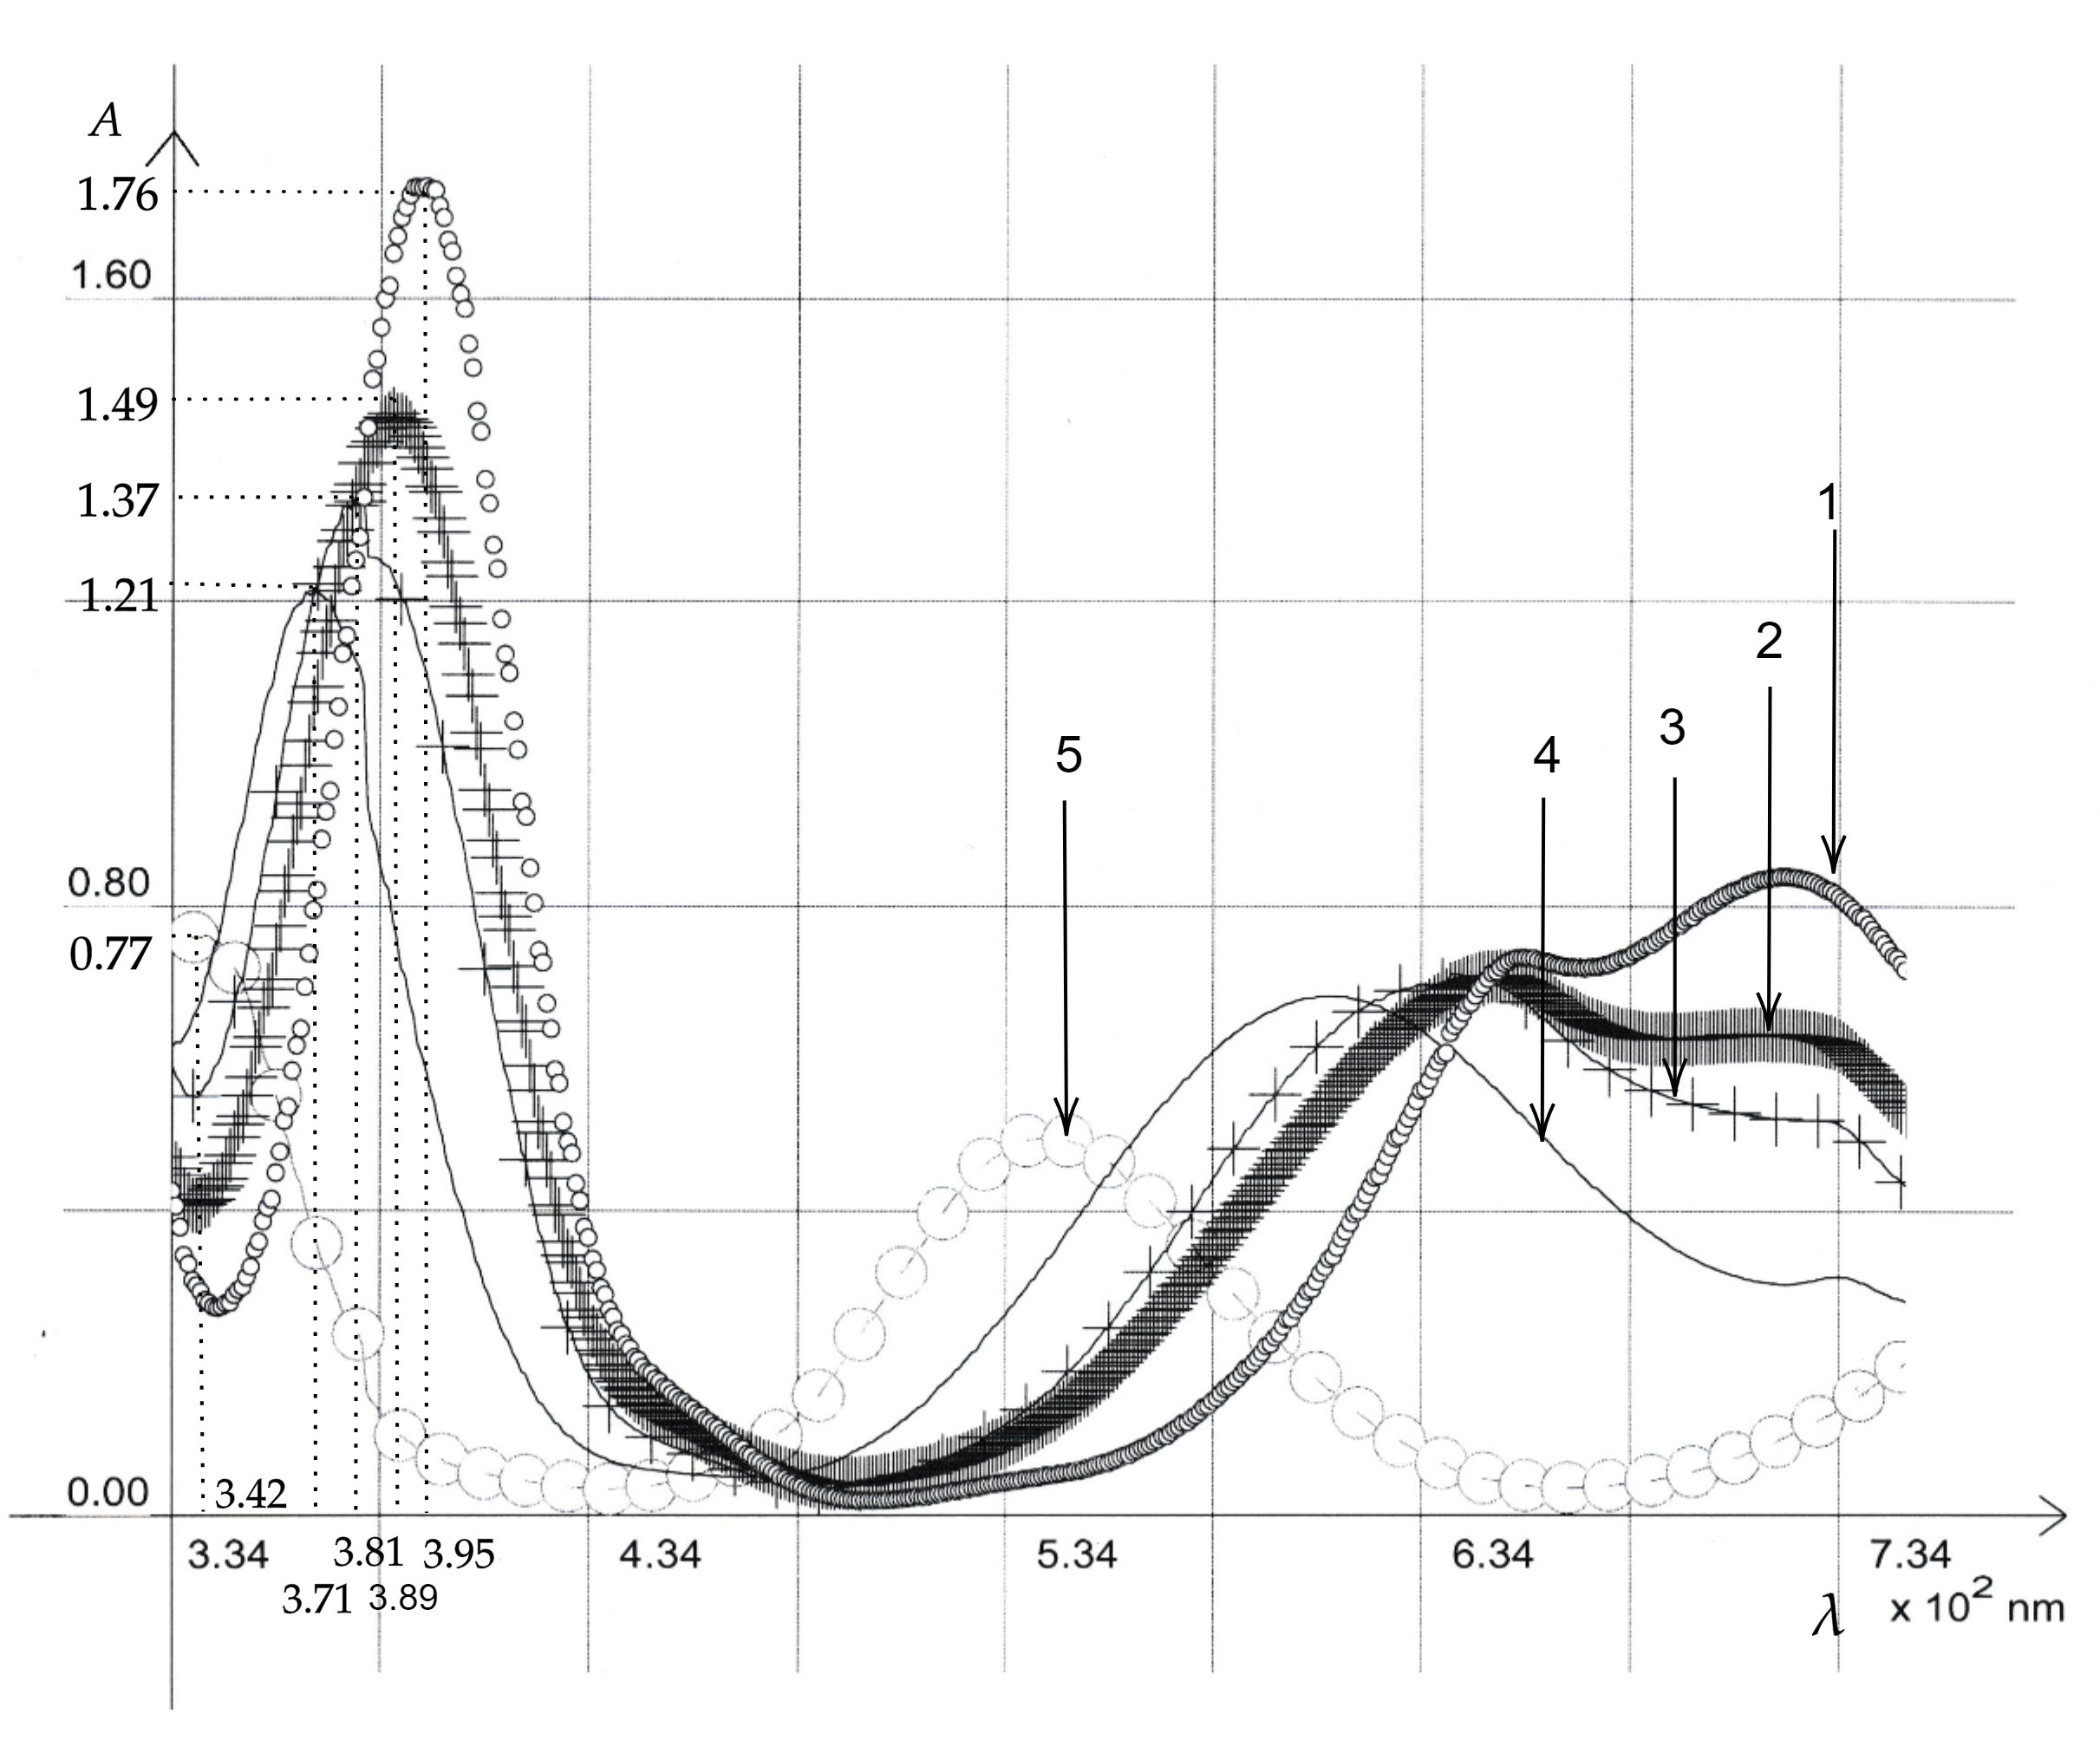
\includegraphics[scale=0.5]{Spectre2_Inorga_bis.jpeg}
        \caption{Spectres d'absorbtion UV-visible des différentes solutions, les numéros des courbes correspondants aux numéros des tubes}
        \label{img2:Spectre_Exp3}
    \end{center}
\end{figure}

\subsection{Théorie et interprétations}

Le nickel peut réaliser plusieurs complexes avec le ligand aqua et le ligand en. 
Il y aura un équilibre entre ces complexes dans les tubes (sauf pour le tube 1 où il n'y a pas de en):
\begin{align*}
    [Ni(H_2O)_6]^{2+} \longleftrightarrow [Ni(H_2O)_4en]^{2+} \longleftrightarrow [Ni(H_2O)_2 (en)_2]^{2+} \longleftrightarrow [Ni(en)_3]^{2+}
\end{align*}

Tous ces complexes sont octaédriques et Ni a toujours un degré d'oxydation $+II$ et un $d^n=d^8$.
Le ligand éthylène diamine est un ligand à champ plus fort que l'eau, avec un $\Delta_O$ plus important.
On s'attend donc à ce que la longueur d'onde diminue lorsque les complexes avec de l'en deviennent majoritaires.


D'après la théorie du champ cristallin, on peut s'attendre à 3 transitions d-d. 
On observe bien 3 pics d'absorbtion pour les courbes, même si le troisième pic de la solution 5 semble coupée, car l'intervalle des longueurs d'ondes est trop faible.

On regroupe nos valeurs de $\lambda_{max}$ et $\epsilon_{max}$ calculées pour chaque tube dans un tableau.

\begin{table}[h!]
    \begin{center}
        \begin{tabular}[pos]{|c|c|c|c|c|c|}
            \hline
            Tube & Couleur solution & $[Ni^{2+}]$ (M) & [en] (M) & $\lambda_{max}$ (nm) & $\epsilon_{max} (L.mol^{-1}.cm^{-1})$ \\
            \hline
            1 &  vert clair & 0.4 & 0 & 395 & 4.4\\
            2 & cyan & 0.32 & 0.08 & 389 & 4.66\\
            3 & bleu & 0.268 & 0.132 & 381 & 5.11\\
            4 & bleu foncé & 0.2 & 0.2 & 371 & 6.05\\
            5 & violet & 0.08 & 0.32 & 342 & 9.63\\
            \hline  
        \end{tabular}
        \caption{Table des valeurs calculés et mesurés pour chaque solution}
        \label{table2:donne3partie}
    \end{center}
\end{table}

Lorsqu'on passe du tube 1 au tube 5 on augmente la concentration en (en) et on diminue la concentration en $Ni^{2+}$. 
On a alors de plus en plus de complexes avec de l'éthylène diamine.
Dans le tube 1 on a que le complexe avec de l'eau et dans le tube 5 on a une majorité de complexe avec 3 en. 
On observe aussi que la longueur d'onde absorbée diminue lorsque la proportion d'en augmente.
Cela est en accord avec nos prédictions, $\Delta_O$ augmente pour les tubes avec une majorité d'éthylène diamine.

\section*{Conclusion}
Dans ce travail pratique, nous avons étudié les couleurs de complexe métallique. Nous
avons déterminé la longueur d'onde absorbée et le coefficient d'extinction molaire de
l'ion permanganate grâce à un spectre d'absorption UV-visible. Nous avons étudié l'effet
de la géométrie du complexe sur la longueur absorbée par des complexes de cobalt. Nous
avons étudié l'effet du champ de ligand sur la couleur d'un complexe de nickel.

\end{document}